\documentclass[11pt,a4paper]{article}
\usepackage[utf8]{inputenc}
\usepackage[german]{babel}
\usepackage{amsmath}
\usepackage{amsfonts}
\usepackage{subfig}
\usepackage{amssymb}
\usepackage{siunitx,physics}
\usepackage{mathtools}
\usepackage{graphicx}
%\usepackage{Here}
\usepackage[version=4]{mhchem}
\usepackage{url}
\usepackage{setspace}
\usepackage[left=2.5cm,right=2.5cm,top=2.5cm,bottom=2cm]{geometry}
[biblography=totocnumbered]
\usepackage{fancyhdr}
\usepackage{scrextend}
\usepackage{hyperref}
\pagenumbering{gobble}

\makeatletter
\newcommand\bigcdot{\mathpalette\bigcdot@{.5}}
\newcommand\bigcdot@[2]{\mathbin{\vcenter{\hbox{\scalebox{#2}{$\m@th#1\bullet$}}}}}
\makeatother

\makeatletter
%\renewcommand*\bib@heading{%
%  \subsection*{}%
%  \@mkboth{\refname}{\refname}}
%\makeatother
\numberwithin{equation}{section}
\numberwithin{figure}{section}

\renewcommand{\labelitemii}{\labelitemfont$\vartriangleright$}
\begin{document}\\
\begin{addmargin}[25pt]{0pt}
Das Phasendiagramm eines binär isomorphen Systems ist in Abbildung \ref{fig:Phasendiagramm_binar_isomorph} dargestellt. Ein binär isomorphes System besteht aus 2 Komponenten, in der Abbildung sind das Kupfer und Nickel. Isomorph bedeutet, dass beide Komponenten sich gut mischen, sowohl im flüssigen als auch im festen Zustand. Die beiden Atomsorten sind im festen Zustand nur gut mischbar wenn ihre Gitterstrukturen gleich sind, sie ähnliche Atomradien haben und sie nicht dazu neigen eine Verbindung einzugehen. Durch die gute Mischbarkeit gibt es nur eine Art der Kristallbildung in der sich dann je nach Zusammensetzung mehr Kupfer oder mehr Nickel befindet. Im Phasendiagramm ist die Zusammensetzung der Mischung gegen die Temperatur aufgetragen, im Diagramm sind dann die Solidus- und die Liquiduslinie eingezeichnet. Unterhalb der Soliduslinie sind nur feste Kristalle möglich, oberhalb der Liquiduslinie nur flüssige Schmelze. Im Bereich zwischen Solidus- und Liquiduslinie können sowohl Schmelze als auch feste Kristalle auftreten, diese Bereich nennt man 2-Phasenbereich.\\
\begin{figure}[h]
    \centering
    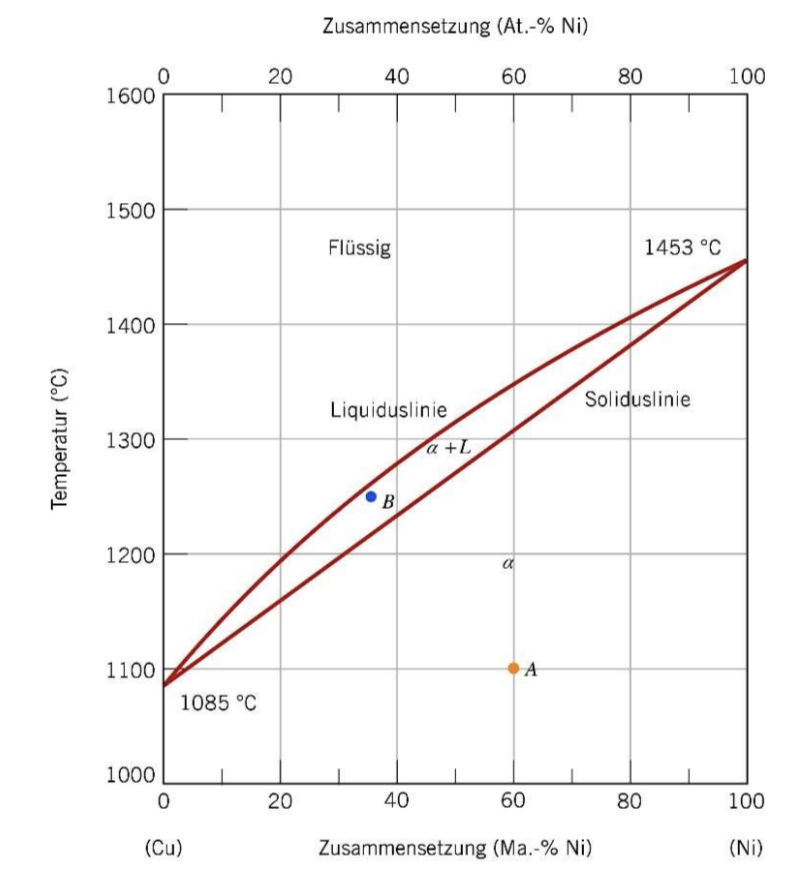
\includegraphics[width = 0.8\textwidth]{images/Materialwissenschaften/Phasendiagramm_binar_isomorph.jpeg}
    \caption{Phasendiagramm eines binär isomorphen System, hier am Beispiel von Kupfer-Nickel}
    \label{fig:Phasendiagramm_binar_isomorph}
\end{figure}
\end{addmargin}


\end{document}